\definecolor{c82b366}{RGB}{130,179,102}
\definecolor{cd5e8d4}{RGB}{213,232,212}
\definecolor{c6c8ebf}{RGB}{108,142,191}
\definecolor{cdae8fc}{RGB}{218,232,252}
\definecolor{c666666}{RGB}{102,102,102}
\definecolor{whitesmoke}{RGB}{245,245,245}
\definecolor{c333333}{RGB}{51,51,51}


\def \globalscale {0.900000}
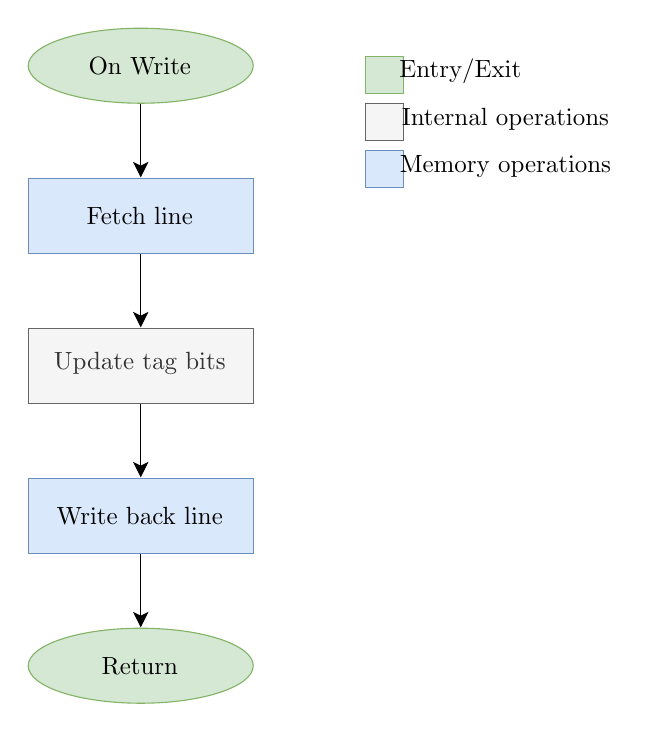
\begin{tikzpicture}[y=1cm, x=1cm, yscale=\globalscale,xscale=\globalscale, every node/.append style={scale=\globalscale}, inner sep=0pt, outer sep=0pt]
  \path[draw=black,miter limit=10.0] (1.5875, 8.4931) -- (1.5875, 7.964) -- (1.5875, 7.6033);



  \path[draw=black,fill=black,miter limit=10.0] (1.5875, 7.4644) -- (1.4949, 7.6496) -- (1.5875, 7.6033) -- (1.6801, 7.6496) -- cycle;



  \path[draw=c82b366,fill=cd5e8d4] (1.5875, 9.0223) ellipse (1.5875cm and 0.5292cm);



  \begin{scope}[fill=black,anchor=south]
    \node[text=black,anchor=south] (text2102) at (1.5743, 8.9032){On Write};



  \end{scope}
  \path[draw=black,miter limit=10.0] (1.5875, 6.3765) -- (1.5875, 5.4867);



  \path[draw=black,fill=black,miter limit=10.0] (1.5875, 5.3478) -- (1.4949, 5.533) -- (1.5875, 5.4867) -- (1.6801, 5.533) -- cycle;



  \path[draw=c6c8ebf,fill=cdae8fc] (0.0, 7.4348) rectangle (3.175, 6.3765);



  \begin{scope}[fill=black,anchor=south]
    \node[text=black,anchor=south] (text2918) at (1.5743, 6.7866){Fetch line};



  \end{scope}
  \path[draw=black,miter limit=10.0] (1.5875, 4.2598) -- (1.5875, 3.7306) -- (1.5875, 3.37);



  \path[draw=black,fill=black,miter limit=10.0] (1.5875, 3.2311) -- (1.4949, 3.4163) -- (1.5875, 3.37) -- (1.6801, 3.4163) -- cycle;



  \path[draw=c666666,fill=whitesmoke] (0.0, 5.3181) rectangle (3.175, 4.2598);



  \begin{scope}[fill=c333333,anchor=south]
    \node[text=c333333,anchor=south] (text5122) at (1.5743, 4.6699){Update tag bits};



  \end{scope}
  \path[draw=black,miter limit=10.0] (1.5875, 2.1431) -- (1.5875, 1.2533);



  \path[draw=black,fill=black,miter limit=10.0] (1.5875, 1.1144) -- (1.4949, 1.2996) -- (1.5875, 1.2533) -- (1.6801, 1.2996) -- cycle;



  \path[draw=c6c8ebf,fill=cdae8fc] (0.0, 3.2015) rectangle (3.175, 2.1431);



  \begin{scope}[fill=black,anchor=south]
    \node[text=black,anchor=south] (text8943) at (1.5743, 2.5532){Write back line};



  \end{scope}
  \path[draw=c82b366,fill=cd5e8d4] (1.5875, 0.5556) ellipse (1.5875cm and 0.5292cm);



  \begin{scope}[fill=black,anchor=south]
    \node[text=black,anchor=south] (text7865) at (1.5743, 0.4366){Return};



  \end{scope}
  \path[draw=c82b366,fill=cd5e8d4] (4.7625, 9.1546) rectangle (5.2917, 8.6254);



  \path (5.1858, 9.2869) rectangle (7.0379, 8.4931);



  \begin{scope}[fill=black,anchor=south]
    \node[text=black,anchor=south] (text8044) at (6.0986, 8.7709){Entry/Exit};



  \end{scope}
  \path[draw=c666666,fill=whitesmoke] (4.7625, 8.4931) rectangle (5.2917, 7.964);



  \path (5.1594, 8.6254) rectangle (8.3344, 7.8317);



  \begin{scope}[fill=black,anchor=south]
    \node[text=black,anchor=south] (text5827) at (6.7336, 8.1095){Internal operations};



  \end{scope}
  \path[draw=c6c8ebf,fill=cdae8fc] (4.7625, 7.8317) rectangle (5.2917, 7.3025);



  \path (5.0271, 7.964) rectangle (8.4667, 7.1702);



  \begin{scope}[fill=black,anchor=south]
    \node[text=black,anchor=south] (text7395) at (6.7336, 7.448){Memory operations};



  \end{scope}

\end{tikzpicture}
